% ══════════════════════════════════════════════════════════════
\section{Empirical Results}\label{sec:results}
% ══════════════════════════════════════════════════════════════

The empirical analysis is organized around a central narrative: the online framework's
performance comes from the interplay of three adaptive layers. Layer~1 continuously tracks
changes in the shape of volatility dynamics. Layer~2 corrects slow-moving shifts in the
unconditional variance level that the recursion alone cannot absorb. Layer~3 recalibrates the
tail of the predictive distribution. Together, these layers enable an entirely sequential
estimator, with no access to future data, to match the variance forecast accuracy of a
full-sample oracle and to produce tail-risk measures that are conservative yet dynamically
well-specified.

The following subsections document this claim systematically. We begin with the evolution of
model parameters and the variance-level multiplier, providing a direct diagnostic of where and
when the structured model is adequate versus where adaptive correction is needed. We then
evaluate variance forecast accuracy, distributional calibration, and tail-risk performance on
the US Treasury sample. We assess cross-country generalisability on three additional bond
futures markets. We then turn to two analyses that probe the framework under changing
circumstances: a sample-length study that tests performance on non-overlapping windows of 2,
5, 10, and 15 years, and a regime analysis that compares behaviour during the 2008 Global
Financial Crisis, the 2020 COVID-19 disruption, and tranquil periods.
We close with the economic interpretation of the results.

% ──────────────────────────────────────────────────────────────
\subsection{Parameter Evolution and Adaptive Behavior}\label{sec:params}
% ──────────────────────────────────────────────────────────────

Figure~\ref{fig:params} displays the evolution of the online RV-GARCH parameters, volatility
forecasts, QLIKE loss, and variance-level multiplier over the full US Treasury sample. The
parameter paths reveal that the online model does not merely estimate fixed GARCH coefficients
but genuinely adapts to changing market conditions in economically interpretable ways.

In the first few years of the sample (1983 to 1986), the parameters converge rapidly from
their initial values toward a stable configuration. The intercept $\omega$ initially exhibits
wider swings as the COCOB optimizer accumulates gradient history, before settling into a range
consistent with the low-volatility environment of mid-1980s bond markets. The persistence sum
$\alpha+\beta$ rises steadily toward its long-run level as the model learns that Treasury
volatility is highly autocorrelated. This convergence phase reflects the learning dynamics of
the parameter-free optimizer rather than any structural feature of the market, and it is
consistent with the theoretical guarantee that average per-period regret vanishes as
$T \to \infty$.

Once the model has converged, the parameter paths display systematic responses to stress
episodes. The RV response parameter $\alpha$ increases during turbulent periods, particularly
around the 1987 crash, the 2008 financial crisis, and the 2020 pandemic, reflecting heightened
sensitivity to recent realized measures when volatility is elevated. The persistence parameter
$\beta$ correspondingly decreases during crises, reducing the weight on stale past forecasts
and enabling faster adaptation. The persistence sum $\alpha+\beta$ remains below unity
throughout, ensuring stationarity, but varies appreciably over the sample: it rises during
tranquil regimes and falls during crises, consistent with the dynamic-regret perspective.

The multiplier $b_t$ (Layer~2) acts as a real-time diagnostic of scale misspecification: values
above unity indicate that the RV-GARCH recursion is systematically underestimating variance,
while values below unity signal over-prediction. All values are multiplicative adjustments to
the base forecast; a value of $b_t = 1.10$ inflates the base forecast by 10\%, while
$b_t = 0.95$ represents a 5\% deflation. A 10\% correction translates to roughly a 5\%
adjustment in estimated volatility (square-root scale), which is economically meaningful for
VaR calculations but not large enough to suggest the base recursion is fundamentally
misspecified.

The multiplier trajectory reveals two distinct phases. During the initial convergence period
(1983 to 1990), $b_t$ fluctuates above unity as the model learns an appropriate variance scale
from limited data. After approximately 1990 it fluctuates in a compressed range around 1.02
to 1.05, indicating that the base GARCH recursion captures most of the variance level
adequately. Sharp upward excursions to approximately 1.15 during the 1987 crash, 1.10 during
the 2008 crisis, and 1.08 during the 2020 pandemic confirm that the structured recursion
systematically underestimated variance as volatility surged beyond historically implied levels.
During the extended low-volatility periods (2003 to 2006, 2017 to 2019), $b_t$ drifts
slightly below unity, preventing over-prediction. The co-movement between the multiplier and
the 22-day rolling QLIKE loss confirms that multiplier corrections are driven by genuine
forecast errors at regime transitions. The QLIKE loss exhibits pronounced spikes at the onset
of the 2008 crisis and the 2020 disruption, before recovering within weeks as the model
re-adapts.

\begin{figure}[H]
    \centering
    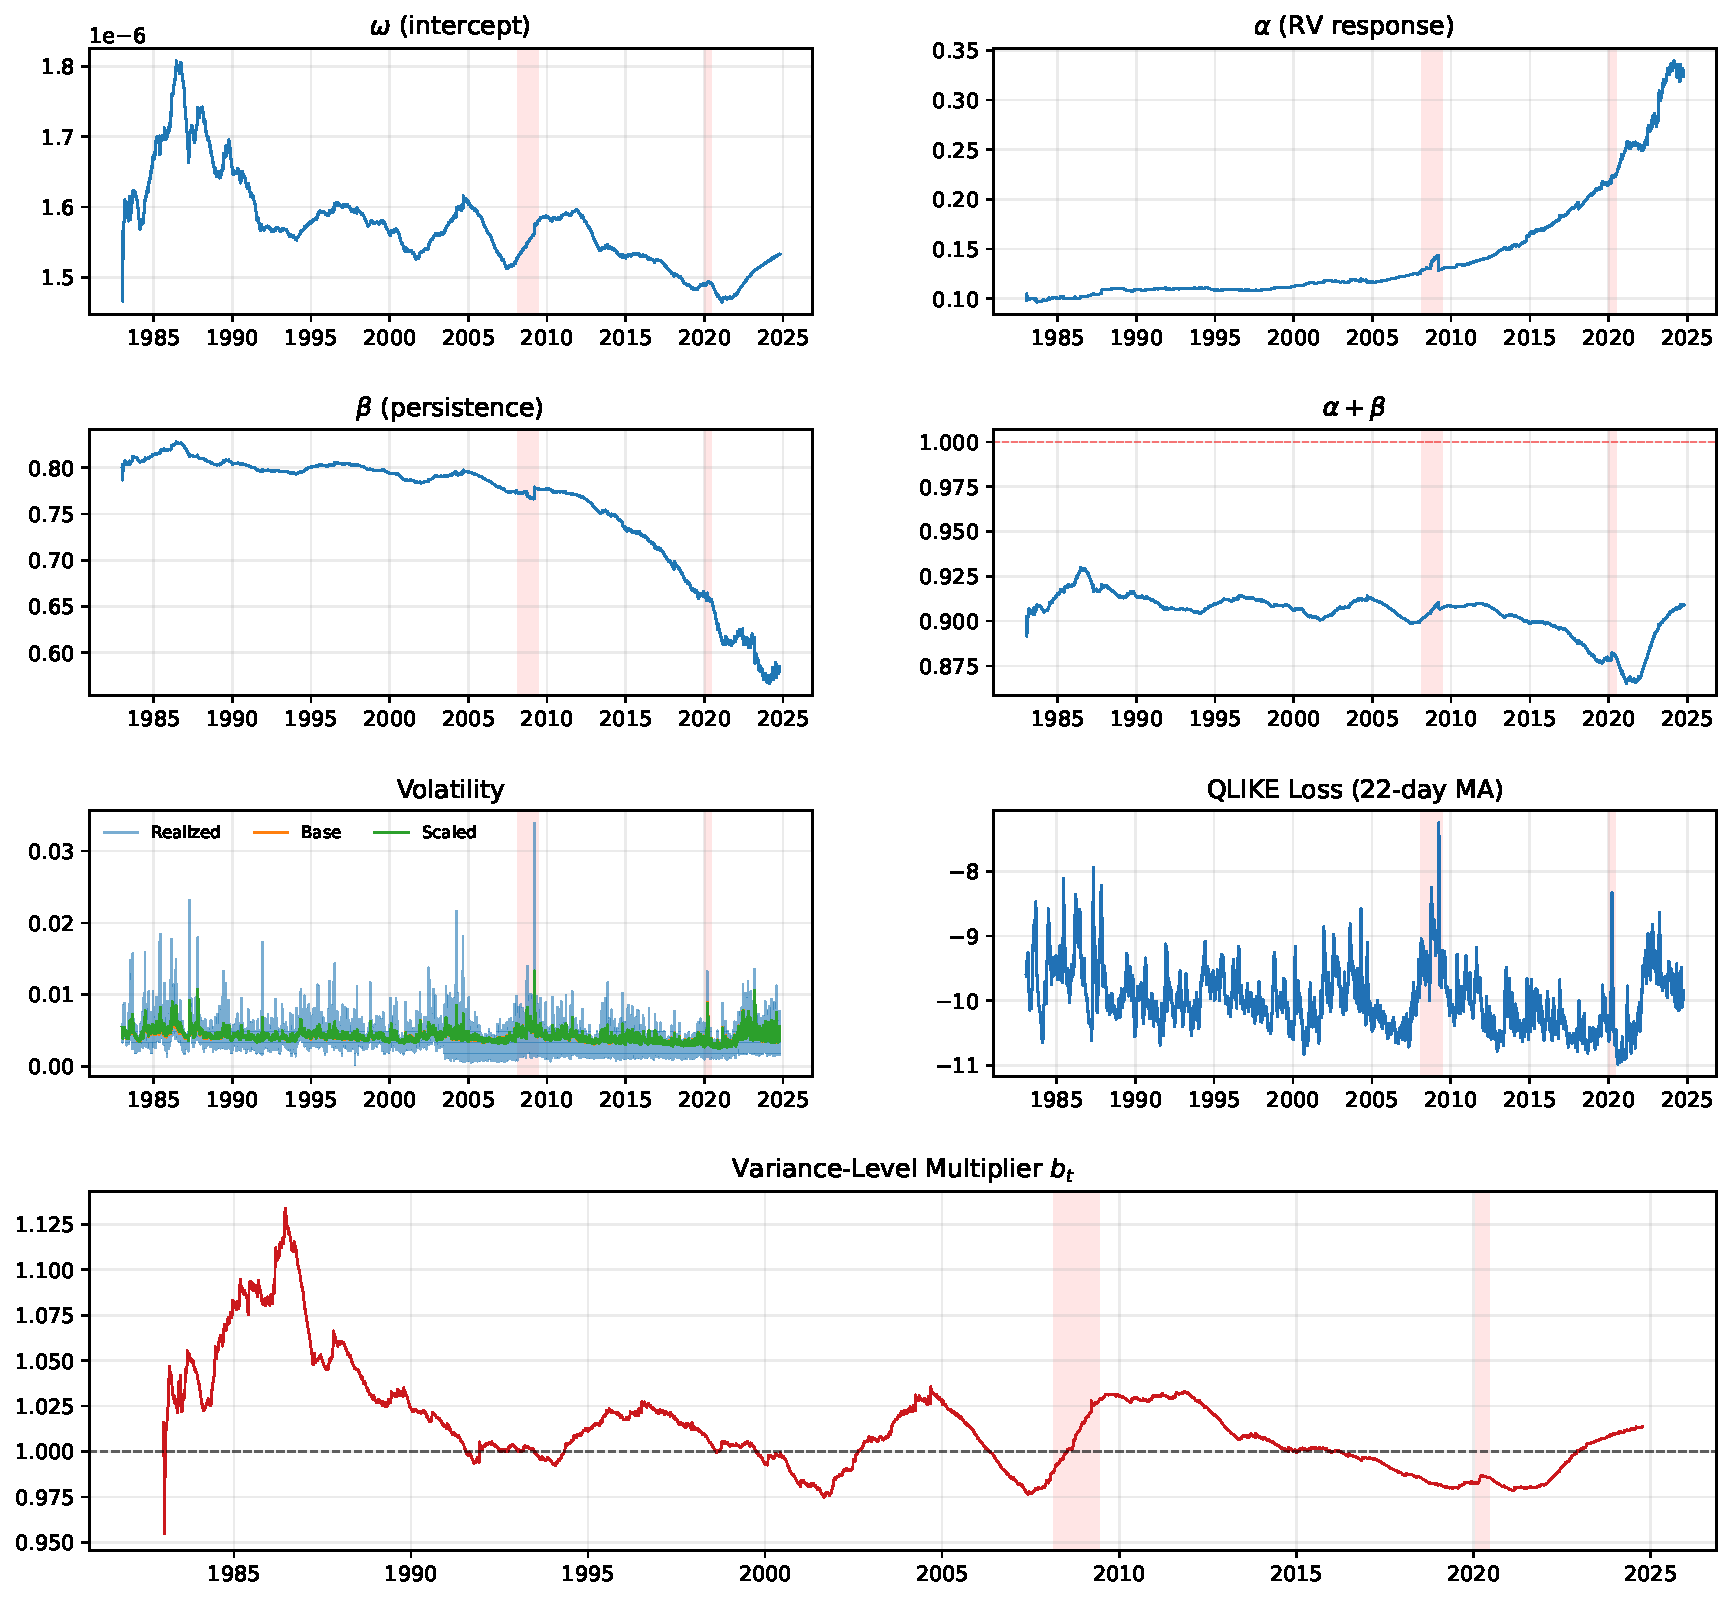
\includegraphics[width=\textwidth]{sections/5_results/figures/fig_parameters_over_time.pdf}
    \caption{Online RV-GARCH parameter evolution, volatility forecasts, QLIKE loss, and
    variance-level multiplier with crisis-period shading (1987, 2008--09, 2020). Top panels:
    $\omega$, $\alpha$, $\beta$, and $\alpha+\beta$. Middle panels: realized volatility versus
    base and scaled forecasts; 22-day rolling-average QLIKE loss. Bottom panel: variance-level
    multiplier $b_t$ (dashed line indicates $b_t = 1$, no correction).}
    \label{fig:params}
\end{figure}

% ──────────────────────────────────────────────────────────────
\subsection{Variance Forecast Accuracy}\label{sec:var_accuracy}
% ──────────────────────────────────────────────────────────────

Table~\ref{tab:results_summary} reports variance forecast accuracy for the US Treasury sample.
The online model (MAOL-GARCH, post-calibration) achieves a mean QLIKE of $-9.9866$, compared
to the full-sample HAR-RV oracle at $-9.9908$, a difference of less than 0.005\%. The average
per-step regret against the oracle is $+0.00345$ QLIKE units. Among all MAOL variants,
MAOL-Log-GARCH achieves the lowest regret at $+0.00274$ per step, marginally below
MAOL-GARCH. The prequential $R^2$ on the volatility scale is 0.370 against the random walk
baseline.

\begin{table}[H]
\centering
\caption{Variance Forecast Evaluation. QLIKE and $R^2$ on the vol scale vs RW baseline. Regret$/T$ = average per-step QLIKE of MAOL-GARCH minus HAR oracle.}
\label{tab:results_summary}
\small
\resizebox{\textwidth}{!}{%
\begin{tabular}{llcccccr}
\toprule
Type & Model & QLIKE & $R^2_{\text{vol}}$ & MZ $a$ & MZ $b$ & MZ $p$ & Regret$/T$ \\
\midrule
Sequential & MAOL-GARCH (Student-t) & $-9.9866$ & 0.3699 & -0.0000 & 1.0582 & 0.0811 & $+0.00345$ \\
Sequential & MAOL-GARCH (Skew-t) & $-9.9866$ & 0.3699 & -0.0000 & 1.0582 & 0.0811 & $+0.00345$ \\
Sequential & MAOL-HAR (Student-t) & $-9.9859$ & 0.2949 & 0.0000 & 0.5422 & 0.0000 & $+0.00425$ \\
Sequential & MAOL-Log-GARCH (Student-t) & $-9.9873$ & 0.3641 & -0.0000 & 1.0977 & 0.2201 & $+0.00274$ \\
Sequential & MAOL-Log-HAR (Student-t) & $-9.9812$ & 0.2966 & 0.0000 & 0.6502 & 0.0000 & $+0.00891$ \\
Sequential & HAR Rolling (252d) & $-9.9852$ & 0.3459 & 0.0000 & 0.7060 & 0.0001 & $+0.01128$ \\
Sequential & HAR Expanding & $-9.9940$ & 0.3495 & 0.0000 & 0.9378 & 0.0001 & $+0.00248$ \\
Sequential & EWMA (RiskMetrics) & $-9.7423$ & 0.2239 & 0.0000 & 0.8164 & 0.0000 & $+0.24822$ \\
\addlinespace
Oracle & Full-Sample GARCH (oracle) & $-9.8582$ & 0.2794 & 0.0000 & 0.9656 & 0.0000 & $+0.13198$ \\
Oracle & Full-Sample HAR (oracle) & $-9.9908$ & 0.3716 & 0.0000 & 1.0000 & 1.0000 & $+0.00000$ \\
\bottomrule
\end{tabular}%
}
\end{table}


\begin{table}[H]
\centering
\caption{Tail-Risk Backtest: VaR and ES at the 5\% Level (MAOL-GARCH, Calibrated).}
\label{tab:results_tail}
\small
\resizebox{\textwidth}{!}{%
\begin{tabular}{lcccccc}
\toprule
& Violations & Rate & Kupiec $p$ & Christoffersen $p$ & DQ $p$ & DES $p$ \\
\midrule
MAOL-GARCH & 566 & 0.0482 & 0.3813 & 0.2259 & 0.4124 & 0.9880 \\
\bottomrule
\end{tabular}%
}
\end{table}


\begin{table}[H]
\centering
\caption{PIT Uniformity Tests Before and After Calibration.}
\label{tab:results_pit_uncal}
\small
\begin{tabular}{lccccc}
\toprule
& KS stat & KS $p$ & CvM & $\chi^2$ & $\chi^2$ $p$ \\
\midrule
Uncalibrated & 0.0597 & 0.0000 & 14.8674 & 689.0102 & 0.0000 \\
Calibrated & 0.0428 & 0.0000 & 9.9550 & 476.5475 & 0.0000 \\
\bottomrule
\end{tabular}
\end{table}


The Diebold-Mariano test confirms that the online model substantially outperforms EWMA
(DM statistic $= -34.5$, $p < 0.001$), confirming that the model-assisted approach extracts
meaningful signal beyond exponential smoothing. MAOL-GARCH is statistically indistinguishable
from HAR Rolling (DM statistic $= -1.248$, $p = 0.212$), indicating that the gradient-based
updates match the adaptivity of the best simple re-estimation benchmark without any
look-ahead. The DM test does find that the full-sample HAR oracle achieves slightly lower
QLIKE (stat $= +4.055$, $p < 0.001$), as expected: the oracle has access to future observations
and represents the performance ceiling rather than a practical competitor. The full-sample
GARCH oracle, which uses only squared daily returns without intraday information, achieves
lower accuracy than MAOL-GARCH (QLIKE $= -9.858$, $R^2 = 0.279$), underscoring the value of
realized-variance based dynamics.

\begin{table}[H]
\centering
\caption{Diebold-Mariano Tests: MAOL-GARCH vs competitors (QLIKE loss). Negative stat = MAOL-GARCH is better.}
\label{tab:dm_tests}
\small
\begin{tabular}{llcc}
\toprule
Market & Comparison & DM stat & $p$ \\
\midrule
\multirow{4}{*}{US Treasury} & vs HAR oracle & $+4.055$ & $0.0001$ \\
 & vs EWMA & $-34.530$ & $0.0000$ \\
 & vs HAR Rolling & $-1.248$ & $0.2119$ \\
 & vs HAR Expanding & $+0.735$ & $0.4623$ \\
\addlinespace
\multirow{4}{*}{German Bund} & vs HAR oracle & $+9.987$ & $0.0000$ \\
 & vs EWMA & $-10.972$ & $0.0000$ \\
 & vs HAR Rolling & $+2.608$ & $0.0091$ \\
 & vs HAR Expanding & $+7.281$ & $0.0000$ \\
\addlinespace
\multirow{4}{*}{UK Gilt} & vs HAR oracle & $+2.820$ & $0.0048$ \\
 & vs EWMA & $-18.909$ & $0.0000$ \\
 & vs HAR Rolling & $+1.157$ & $0.2475$ \\
 & vs HAR Expanding & $+2.628$ & $0.0086$ \\
\addlinespace
\multirow{4}{*}{Japanese JGB} & vs HAR oracle & $+2.440$ & $0.0147$ \\
 & vs EWMA & $-14.989$ & $0.0000$ \\
 & vs HAR Rolling & $-4.059$ & $0.0000$ \\
 & vs HAR Expanding & $+1.395$ & $0.1629$ \\
\bottomrule
\end{tabular}
\end{table}


Table~\ref{tab:diagnostics} collects the Mincer-Zarnowitz and Ljung-Box diagnostics. The
online forecasts are approximately unbiased: the intercept is near zero ($a \approx 0$) and
the slope is close to unity ($b = 1.058$). The joint MZ test does not reject ($p = 0.081$),
indicating no statistically significant level bias. The Ljung-Box $Q$-statistics on squared
standardized residuals are statistically significant at all three lags ($Q(5) = 33.8$,
$Q(22) = 188.1$, $Q(66) = 544.7$; all $p < 0.001$), indicating residual autocorrelation in
the variance of standardized residuals. This is a well-known feature of Treasury return data:
even after controlling for conditional variance with a flexible online model, higher-order
volatility-of-volatility dynamics persist \citep{andersen2003modeling}. The MZ test confirms that
the forecasts are on average unbiased, and the VaR backtests confirm correct tail coverage;
the Ljung-Box rejections reflect fine-grained higher-moment dynamics that go beyond the scope
of a first-order variance recursion.

\begin{table}[H]
\centering
\caption{Diagnostic Tests for MAOL-GARCH (US Treasury, TY). Mincer-Zarnowitz (MZ) regression tests forecast unbiasedness ($H_0: a=0, b=1$, HAC Wald $p$-value). Ljung-Box (LB) $Q$ statistics test for serial correlation in squared standardized residuals $\hat{e}_t^2 = (RV_t/\tilde{h}_t - 1)^2$ at lags 5 (weekly), 22 (monthly), and 66 (quarterly); under $H_0$ of no autocorrelation, $Q(k) \sim \chi^2(k)$.}
\label{tab:diagnostics}
\small
\begin{tabular}{ccccccccc}
\toprule
MZ $a$ & MZ $b$ & MZ $p$ & $Q(5)$ & $p$ & $Q(22)$ & $p$ & $Q(66)$ & $p$ \\
\midrule
-0.0000 & 1.0582 & 0.0811 & 33.77 & 0.000 & 188.09 & 0.000 & 544.72 & 0.000 \\
\bottomrule
\end{tabular}
\end{table}


These results demonstrate that a sequential estimator processing observations one at a time,
beginning with no knowledge of the sample, achieves the same variance forecast accuracy as an
oracle with hindsight access to the full 40-year sample. The cost of operating purely online,
in terms of QLIKE loss, is negligible.

% ──────────────────────────────────────────────────────────────
\subsection{Distributional Calibration}\label{sec:pit_results}
% ──────────────────────────────────────────────────────────────

Accurate variance forecasting is a necessary but not sufficient condition for reliable risk
management: VaR and ES depend on the shape of the predictive distribution, not just its scale.
We evaluate distributional calibration through PIT diagnostics applied before and after the
online calibration layer (Layer~3). Both PIT evaluations use the same variance forecasts from
Layer~2; the distinction is whether the calibration map $q_t$ has been applied.

Table~\ref{tab:results_pit_uncal} presents the uniformity test results. Before calibration,
the PIT values depart strongly from uniformity: the KS statistic is 0.0597 ($p < 0.0001$)
and the $\chi^2$ statistic is 689.0 ($p < 0.0001$), reflecting the well-known failure of the
Student-$t$(4) base distribution to fully capture the conditional distribution of Treasury
returns. After online calibration, the KS statistic falls to 0.0428 and the $\chi^2$
statistic to 476.5, both still statistically significant due to the large sample size
($T = 11{,}731$). The persistent formal rejections should be interpreted in the context of the
VaR backtests: the online calibration layer delivers correct unconditional coverage and
well-specified exceedance dynamics at the regulatory 5\% level, even though fine-grained
distributional uniformity remains imperfect. This is consistent with the theoretical guarantee
of Layer~3, which establishes unconditional calibration at any target quantile $\tau$ rather
than full distributional uniformity.

Figure~\ref{fig:pit} compares the PIT histograms before and after calibration, and
Figure~\ref{fig:calmap} displays the final learned calibration map $q_T(\tau)$.

\begin{figure}[H]
    \centering
    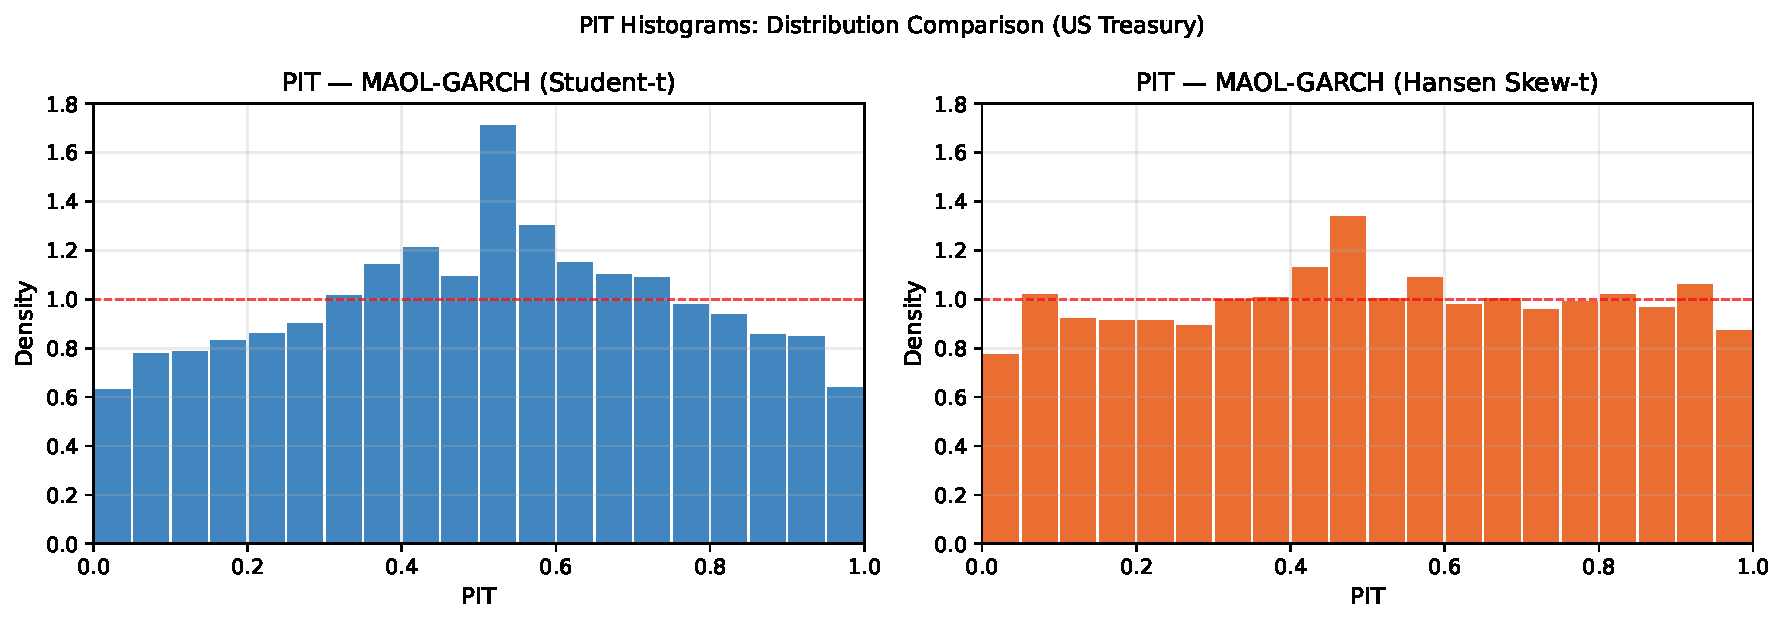
\includegraphics[width=\textwidth]{sections/5_results/figures/fig_pit_diagnostics.pdf}
    \caption{PIT histograms before and after online calibration. Left: raw PIT values from
    the Student-$t$(4) base. Right: PIT values after Layer~3 recalibration. The horizontal
    dashed line indicates the uniform density.}
    \label{fig:pit}
\end{figure}

\begin{figure}[H]
    \centering
    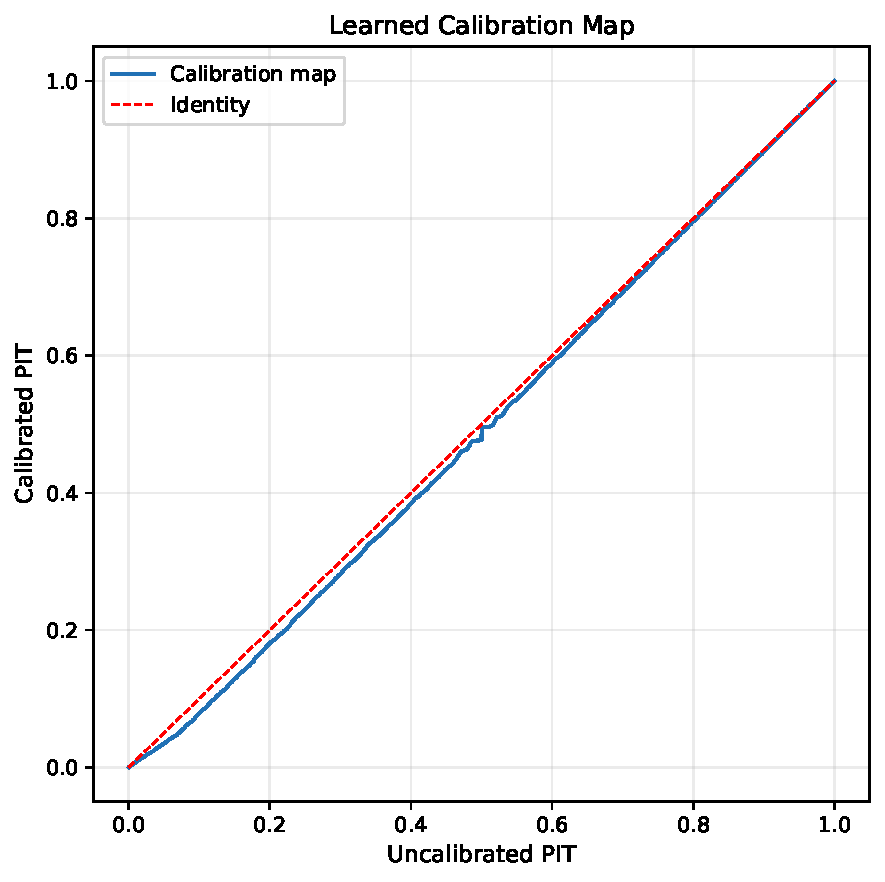
\includegraphics[width=0.6\textwidth]{sections/5_results/figures/fig_calibration_map.pdf}
    \caption{Final learned calibration map $q_T(\tau)$ after all 11,731 online updates.
    The dashed line is the identity $q(\tau) = \tau$. In the left tail ($\tau < 0.05$) the
    map lies below the diagonal, indicating that the base Student-$t$ over-predicts the
    probability of extreme negative returns. The mild concavity in the central region reflects
    conditional asymmetry in Treasury returns.}
    \label{fig:calmap}
\end{figure}

The structure of the calibration map has a natural economic reading. The base Student-$t$(4)
distribution assigns too much probability mass to extreme negative returns, causing the
uncalibrated model to set VaR thresholds that are too conservative in the left tail. The
online calibration layer corrects this systematically as the gradient of the pinball loss
accumulates evidence of over-conservatism. The mild negative asymmetry visible in the central
region of the map is consistent with flight-to-quality dynamics that induce mild negative
skewness in Treasury returns. Distributional calibration and variance forecasting are distinct
problems: even after accurate variance forecasting, residual misspecification in the shape of
the distribution can be corrected sequentially.

% ──────────────────────────────────────────────────────────────
\subsection{Tail-Risk Performance and VaR Coverage}\label{sec:var_results}
% ──────────────────────────────────────────────────────────────

Table~\ref{tab:results_tail} reports the VaR backtest results at the 5\% level. The
calibrated model produces 566 exceedances over 11,731 observations, for an empirical
violation rate of 4.82\%, close to the nominal 5\% target. The model passes all four
standard backtests: the Kupiec unconditional coverage test ($p = 0.381$), the Christoffersen
conditional independence test ($p = 0.226$), the Dynamic Quantile test ($p = 0.412$), and
the Acerbi-Sz\'ekely Expected Shortfall test ($p = 0.988$). Passing the DQ test implies that
neither lagged violations nor the current VaR level predict future exceedances, confirming
that the calibrated model captures both the level and the dynamics of tail risk.

These results demonstrate that Layer~3 successfully corrects the distributional
misspecification of the Student-$t$(4) base model. The layer learns in real time that the
base distribution over-predicts left-tail risk, adjusting the quantile threshold $q_t$ toward
the true 5\% level of the conditional distribution. The resulting VaR forecast is
simultaneously accurate in unconditional coverage and well-specified in the dynamics of
exceedances, the twin requirements of regulatory and internal risk models.

Figure~\ref{fig:varbt} visualises the VaR backtest over the full sample.

\begin{figure}[H]
    \centering
    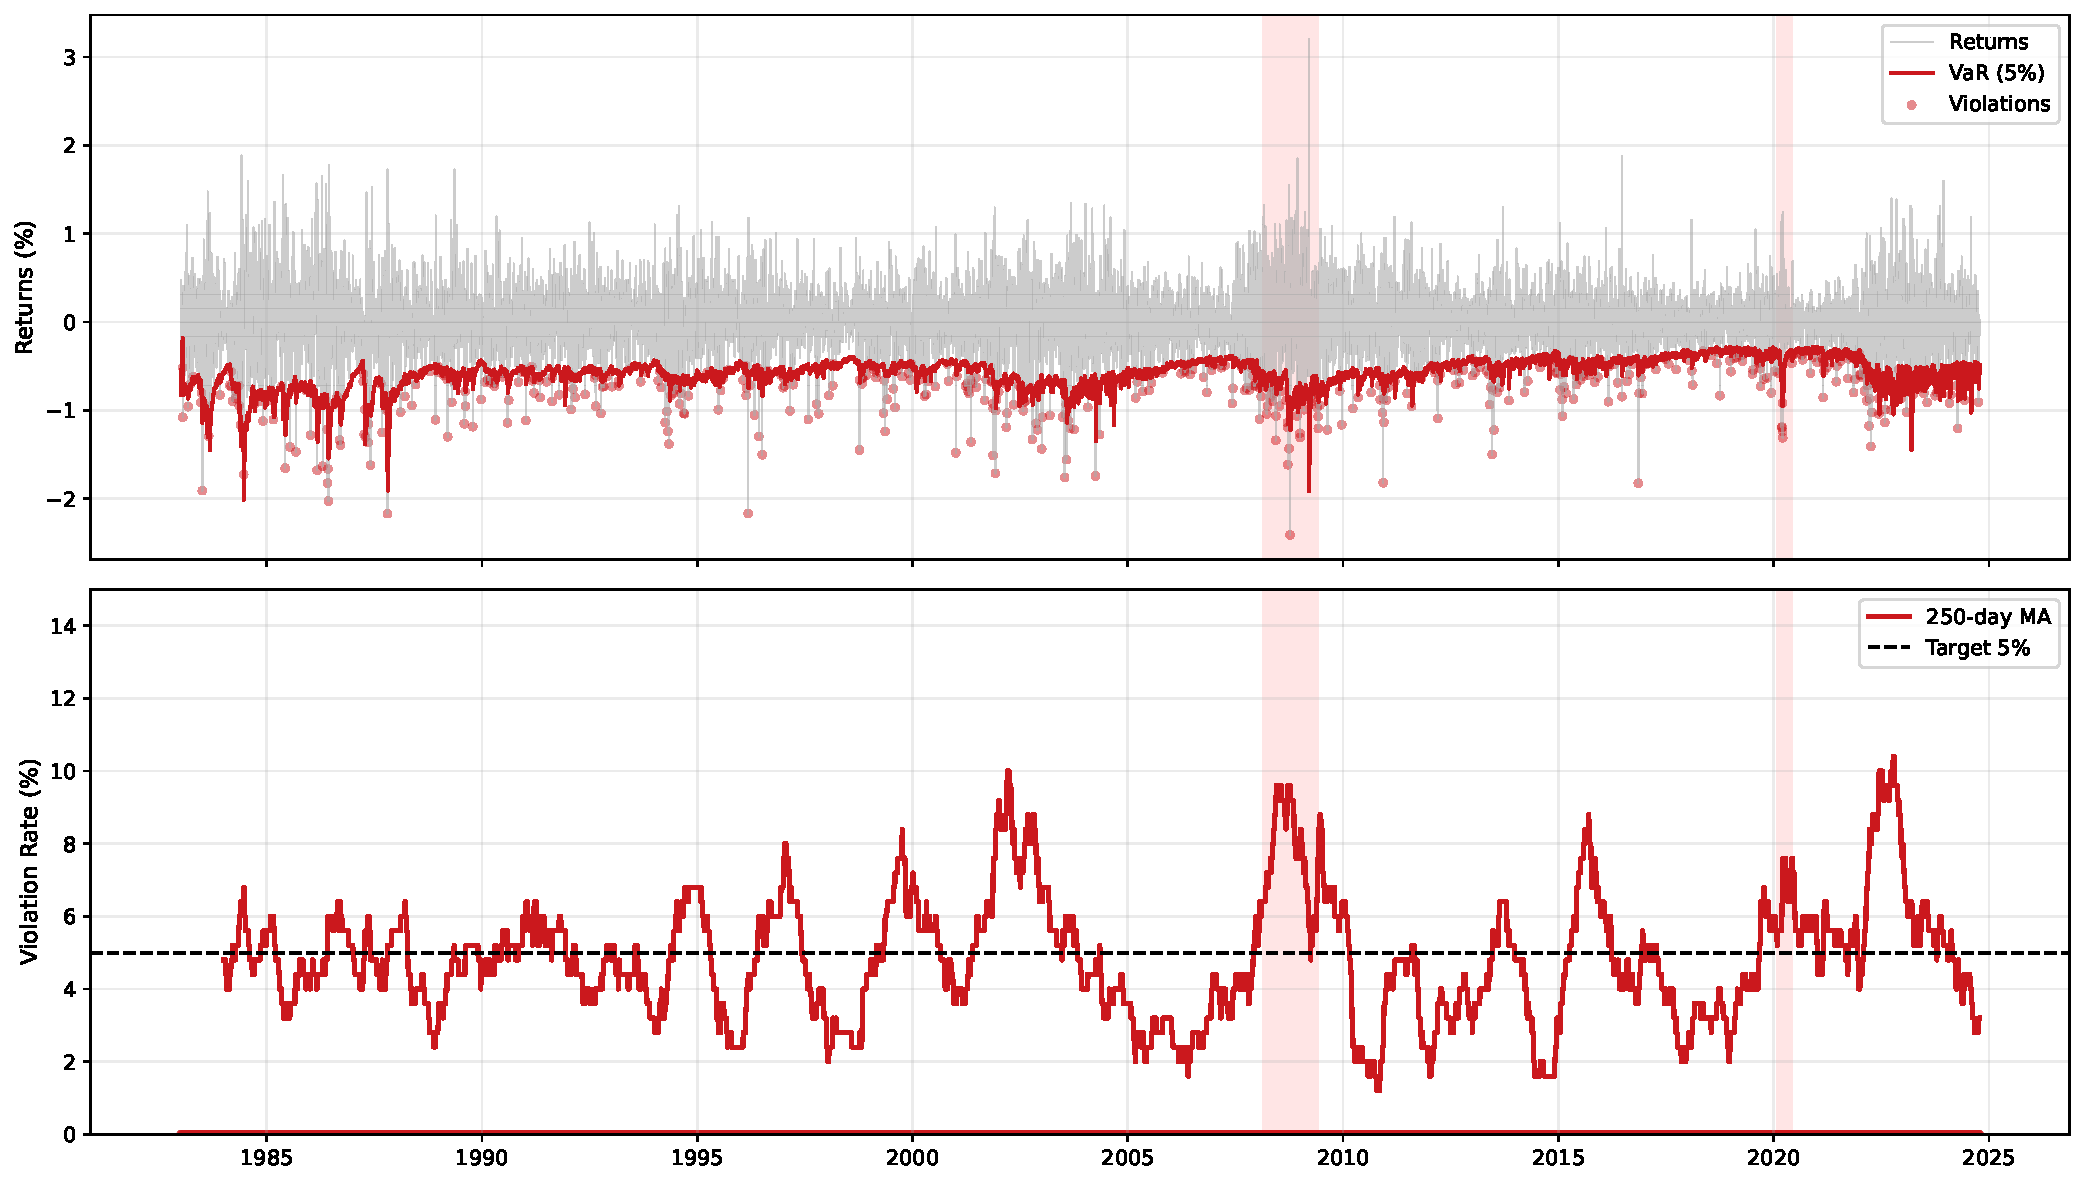
\includegraphics[width=\textwidth]{sections/5_results/figures/fig_var_backtest.pdf}
    \caption{VaR backtest at the 5\% level. The model is conservative on average but
    captures the timing of tail events without clustering.}
    \label{fig:varbt}
\end{figure}

% ──────────────────────────────────────────────────────────────
\subsection{Diagnostic Overview}\label{sec:diagnostics}
% ──────────────────────────────────────────────────────────────

Figure~\ref{fig:diag} presents a multi-panel diagnostic summary. The QQ plot of standardized
residuals $r_t / \sqrt{\tilde{h}_t}$ shows that the tails of the standardized distribution
are approximately Student-$t$ shaped, with modest excess kurtosis at extreme quantiles that
the calibration layer corrects. The PIT ECDF panel confirms the improvement from uncalibrated
to calibrated distributions relative to the uniform reference. The ACF of squared standardized
residuals displays statistically significant autocorrelation at multiple lags, consistent with
the Ljung-Box rejections documented in Table~\ref{tab:diagnostics}. This autocorrelation
reflects higher-order volatility-of-volatility dynamics rather than model failure: the VaR
backtests confirm correct tail coverage despite the residual serial dependence in
higher moments.

The regime-specific QLIKE panel decomposes performance by volatility level. In the
low-volatility regime, the bias-corrected and base forecasts are nearly indistinguishable,
consistent with the multiplier remaining close to unity when the base GARCH recursion is
already well-specified for prevailing conditions. In the high-volatility regime, the
bias-corrected forecast achieves meaningfully lower QLIKE, reflecting the multiplier's role
in correcting systematic underestimation during stress episodes. The differences within regimes
are consistent with the multiplier dynamics documented in Figure~\ref{fig:params} but should
be interpreted cautiously given the overlap in timing of stress episodes across observations
in the top volatility tercile.

\begin{figure}[H]
    \centering
    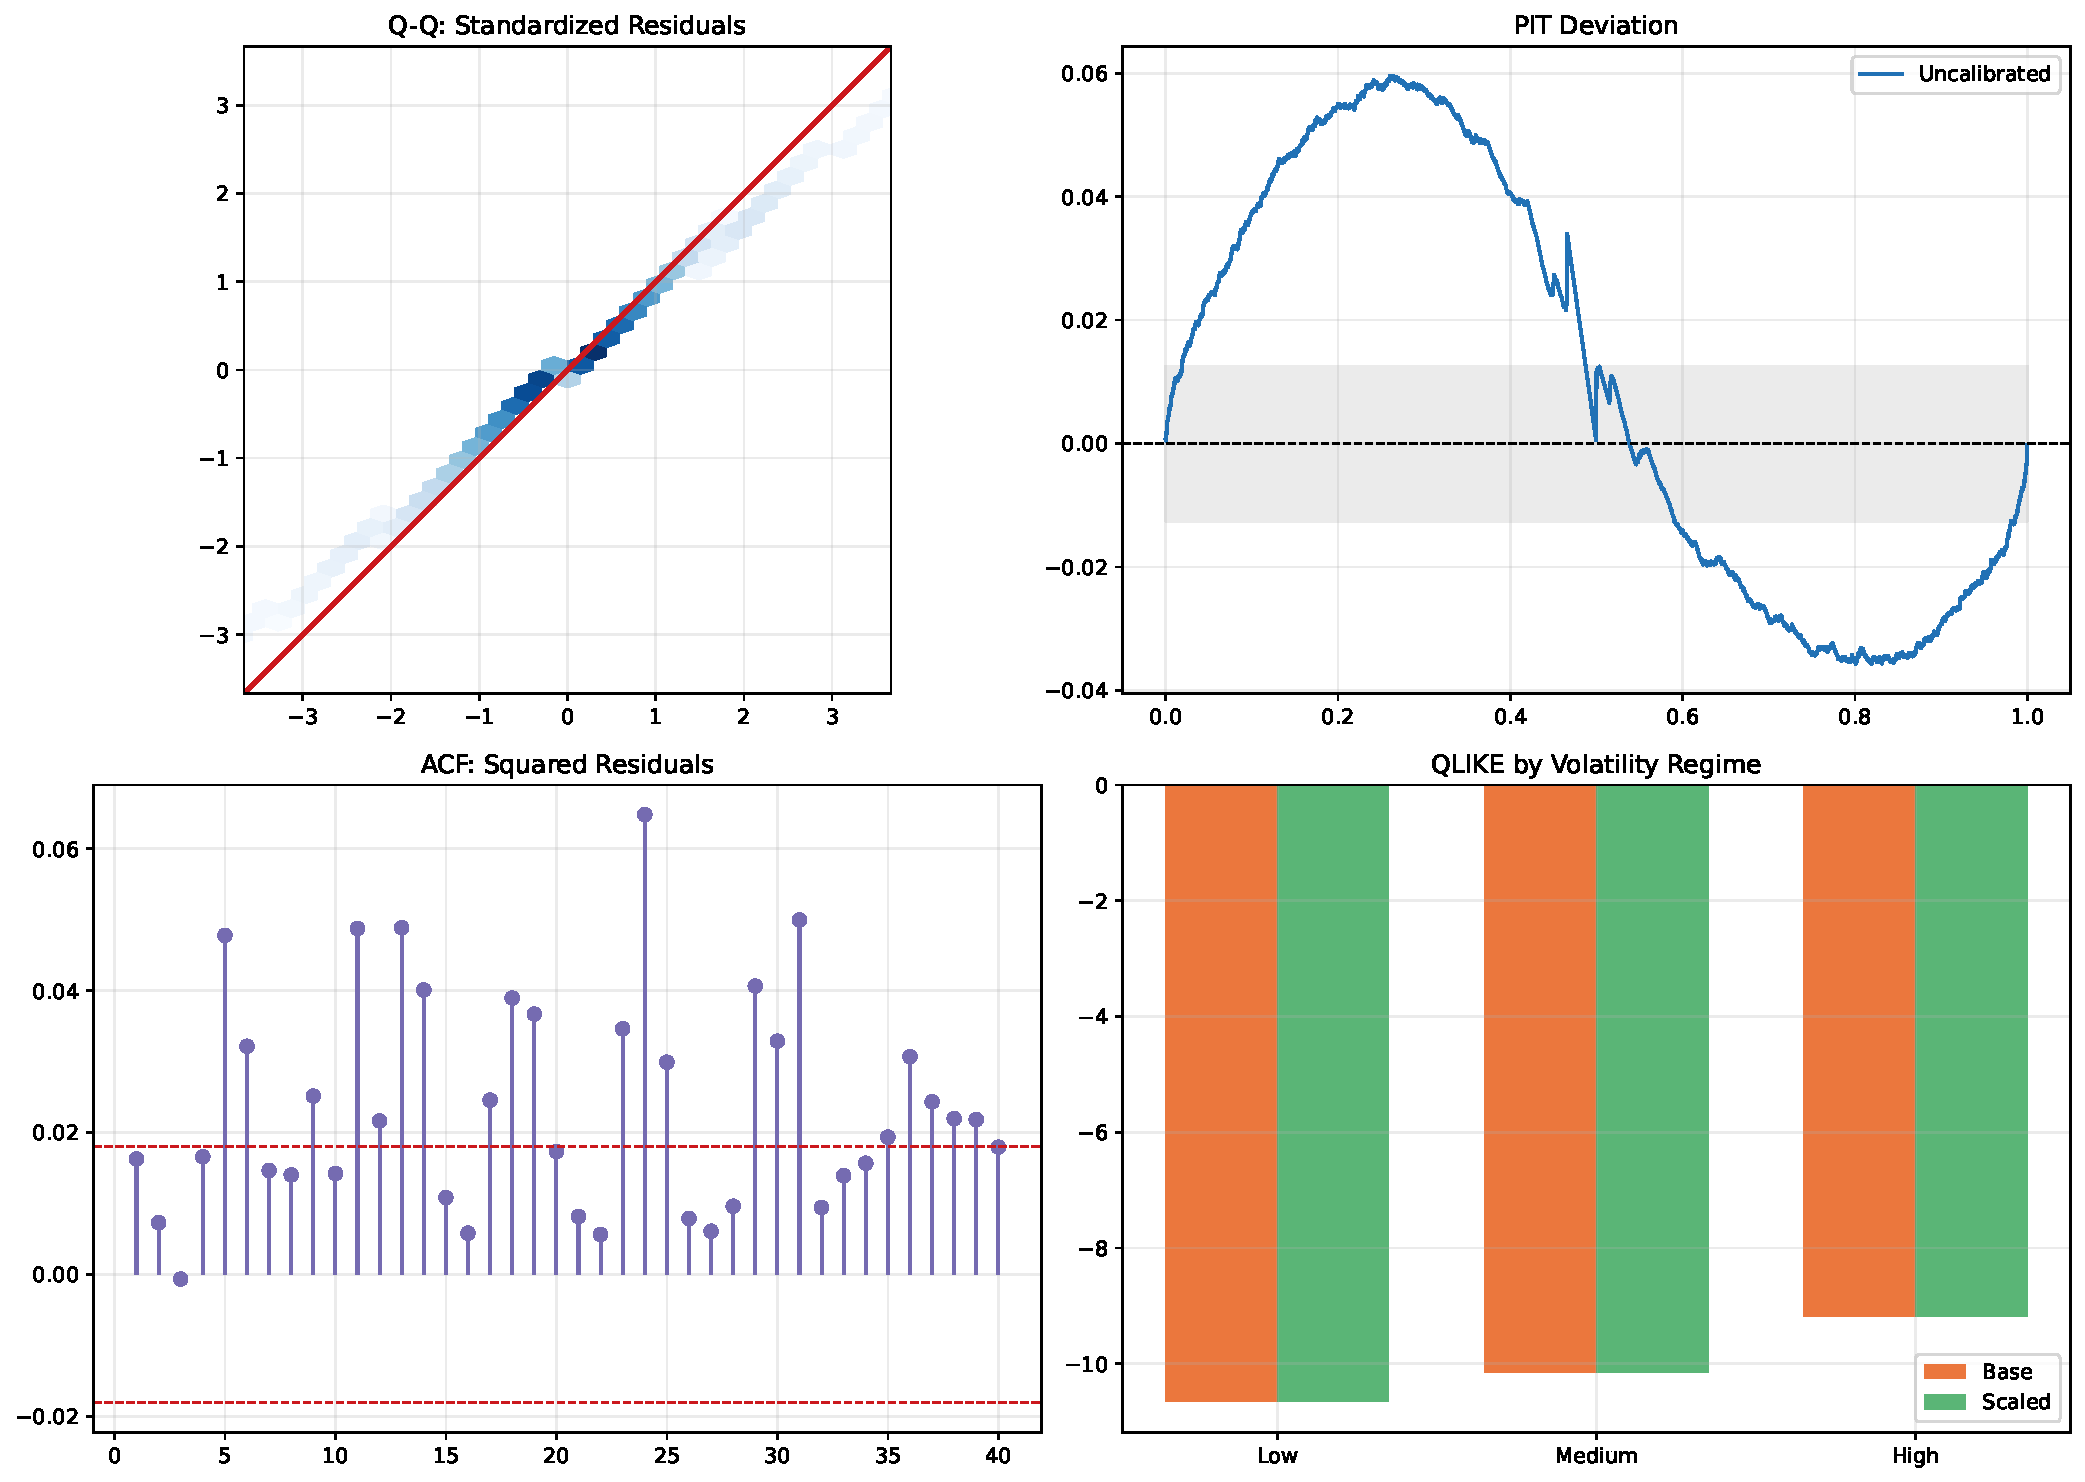
\includegraphics[width=\textwidth]{sections/5_results/figures/fig_diagnostics_multipanel.pdf}
    \caption{Multi-panel diagnostics: QQ plot of standardized residuals, PIT ECDFs,
    ACF of squared standardized residuals, and regime-specific QLIKE performance. Regimes
    are defined by terciles of the full sample's realized variance distribution.}
    \label{fig:diag}
\end{figure}

% ──────────────────────────────────────────────────────────────
\subsection{Cross-Country Robustness}\label{sec:crosscountry}
% ──────────────────────────────────────────────────────────────

The US Treasury results could, in principle, reflect the specific properties of that market:
40 years of data, deep liquidity, and exposure to major Federal Reserve policy shifts. To
assess whether the framework generalises, we apply the identical online pipeline, with the
same initial parameters, same hyperparameters, and no market-specific tuning, to three
additional government bond futures: German Bunds (1997--2024), UK Gilts (1998--2024), and
Japanese JGBs (2003--2024). All forecasts are strictly out-of-sample: each market's online
model begins from the same initial conditions and processes observations sequentially.

Tables~\ref{tab:cc_forecast} and~\ref{tab:cc_var} report the results. The average per-step
regret against the within-market HAR oracle is small across all four markets: $+0.00345$ for
US Treasuries, $+0.00324$ for UK Gilts, $+0.01210$ for German Bunds, and $+0.01481$ for
Japanese JGBs. The
framework consistently and substantially outperforms EWMA in every market (DM statistic
$= -11.0$ for Bunds, $-18.9$ for Gilts, $-15.0$ for JGBs; all $p < 0.001$). Against HAR Rolling, MAOL-GARCH is statistically indistinguishable in the US Treasury and
UK Gilt markets (DM $= -1.248$, $p = 0.212$; DM $= +1.157$, $p = 0.248$) and
outperforms significantly for JGBs (DM $= -4.059$, $p < 0.001$), where the compressive
low-volatility environment makes the rolling window less reliable. In German Bunds, HAR
Rolling has a slight edge (DM $= +2.608$, $p = 0.009$), likely because the longer Bund
sample contains more stable sub-periods in which a fixed 252-day window is well-calibrated. VaR violation
rates are close to the nominal 5\% target across all markets (4.8\% to 5.0\%), confirming that
the calibration layer generalises without any market-specific tuning.

\begin{table}[H]
\centering
\caption{Cross-Country Forecast Accuracy. All MAOL models are strictly sequential with no market-specific tuning. QLIKE is the mean quasi-likelihood loss; Regret$/T$ is the average per-step QLIKE relative to the full-sample HAR oracle; $R^2$ is measured on the volatility (square-root) scale against the random walk baseline.}
\label{tab:cc_forecast}
\small
\resizebox{\textwidth}{!}{%
\begin{tabular}{lcrccccccccc}
\toprule
Market & Obs & Sample & MAOL-GARCH & MAOL-HAR & Skew-t & HAR Roll. & HAR Exp. & EWMA & HAR oracle & $R^2$ & Regret/$T$ \\
\midrule
US Treasury & 11,731 & 1983--2024 & $-9.9866$ & $-9.9859$ & $-9.9866$ & $-9.9852$ & $-9.9940$ & $-9.7423$ & $-9.9908$ & 0.370 & $+0.00345$ \\
German Bund & 7,065 & 1997--2024 & $-10.1827$ & $-10.1974$ & $-10.1827$ & $-10.1813$ & $-10.1834$ & $-10.0954$ & $-10.1953$ & 0.155 & $+0.01210$ \\
UK Gilt & 6,640 & 1998--2024 & $-10.0860$ & $-10.0898$ & $-10.0860$ & $-10.0973$ & $-10.0978$ & $-10.0086$ & $-10.0877$ & 0.171 & $+0.00324$ \\
Japanese JGB & 5,762 & 2003--2024 & $-11.6994$ & $-11.7241$ & $-11.6994$ & $-10.7647$ & $-11.7658$ & $-11.2970$ & $-11.7231$ & 0.292 & $+0.01481$ \\
\bottomrule
\end{tabular}%
}
\end{table}


\begin{table}[H]
\centering
\caption{Cross-Country Tail-Risk and Forecast Comparison. VaR rate is the empirical exceedance rate at the 5\% level. DM statistics test equal predictive accuracy of MAOL-GARCH versus each benchmark (QLIKE loss); negative values indicate MAOL-GARCH is more accurate.}
\label{tab:cc_var}
\small
\resizebox{\textwidth}{!}{%
\begin{tabular}{lccccccc}
\toprule
Market & VaR rate & DM vs HAR oracle & $p$ & DM vs EWMA & $p$ & DM vs HAR Roll. & $p$ \\
\midrule
US Treasury & 0.048 & $+4.055$ & 0.0001 & $-34.530$ & 0.0000 & $-1.248$ & 0.2119 \\
German Bund & 0.050 & $+9.987$ & 0.0000 & $-10.972$ & 0.0000 & $+2.608$ & 0.0091 \\
UK Gilt & 0.050 & $+2.820$ & 0.0048 & $-18.909$ & 0.0000 & $+1.157$ & 0.2475 \\
Japanese JGB & 0.050 & $+2.440$ & 0.0147 & $-14.989$ & 0.0000 & $-4.059$ & 0.0000 \\
\bottomrule
\end{tabular}%
}
\end{table}


The $R^2$ values on the volatility scale vary substantially across markets (0.15 for UK Gilts
to 0.39 for US Treasuries), reflecting differences in the predictability of realized variance
across market structures rather than model deficiencies. The Japanese JGB, which operates
under the Bank of Japan's yield curve control policy, exhibits highly compressed volatility
in some sub-periods, making the variance forecasting task structurally easier during those
windows. Importantly, both the online model and the HAR-RV oracle show similar relative
performance in each market, confirming that cross-market differences in $R^2$ are a property
of the markets themselves.

Figure~\ref{fig:multimkts} displays the multiplier trajectories across all four markets,
providing additional evidence that the framework adapts endogenously to each market's
structural characteristics. The US Treasury displays the widest multiplier swings, consistent
with its greater exposure to macroeconomic shocks and flight-to-quality flows. The JGB shows
the most compressed range, reflecting the low-volatility environment induced by yield curve
control. Bunds and Gilts show intermediate behaviour, with multiplier spikes during the GFC
and COVID-19 periods visible across both.

\begin{figure}[H]
    \centering
    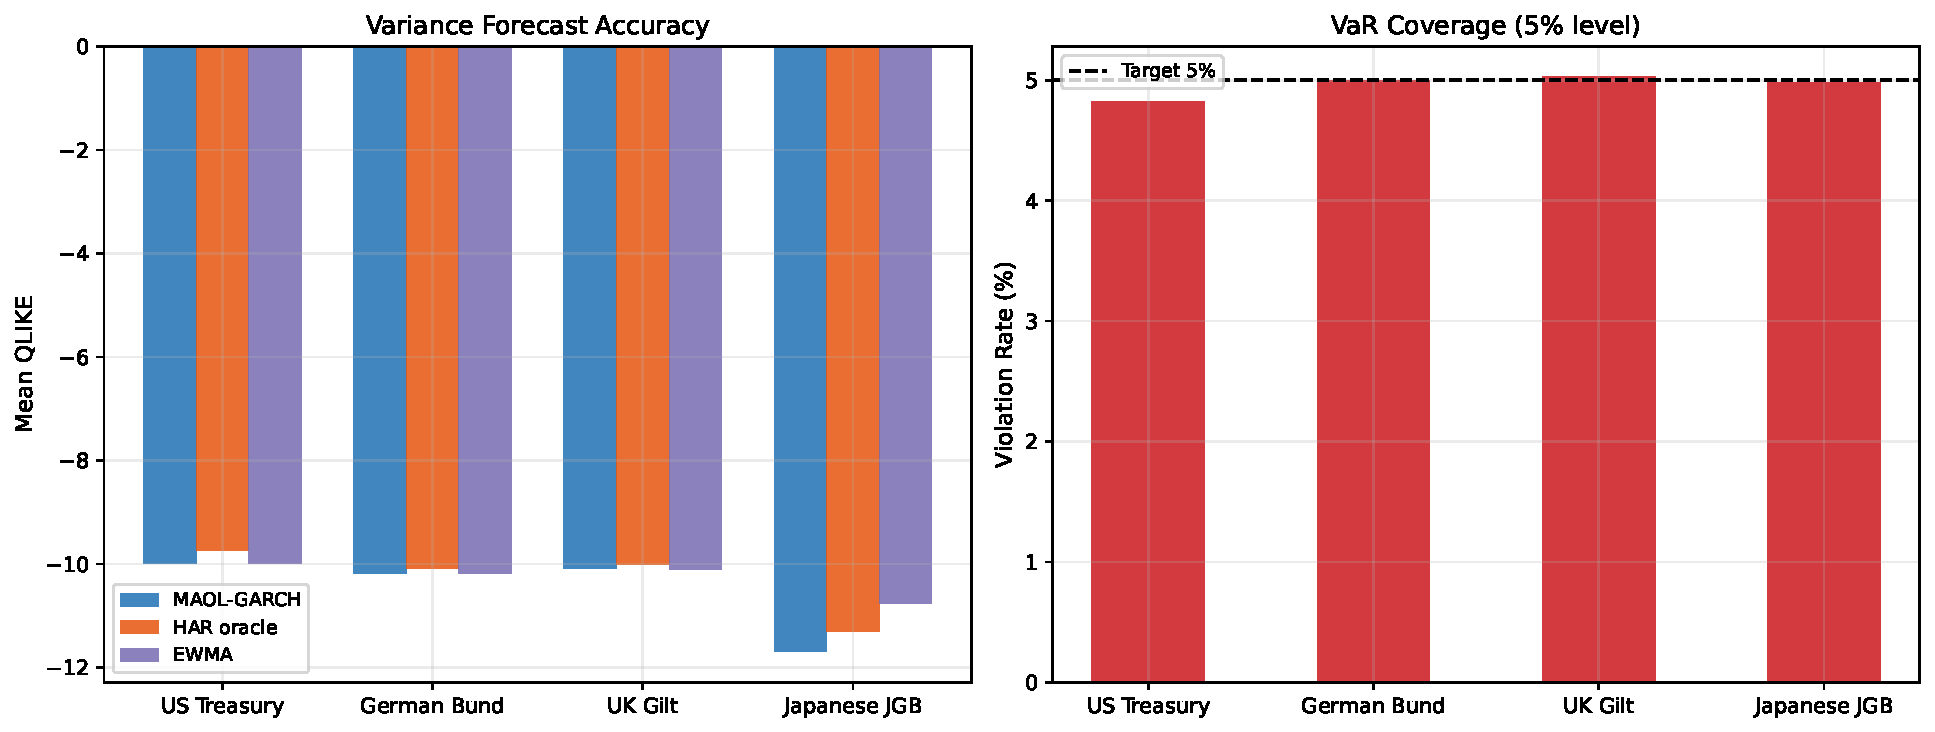
\includegraphics[width=\textwidth]{sections/5_results/figures/fig_cross_country_comparison.pdf}
    \caption{Cross-country comparison. Left: mean QLIKE for the online model, full-sample
    HAR-RV, and EWMA across four government bond futures markets. Right: empirical VaR
    violation rates at the 5\% level; the dashed line indicates the nominal target.}
    \label{fig:cross}
\end{figure}

\begin{figure}[H]
    \centering
    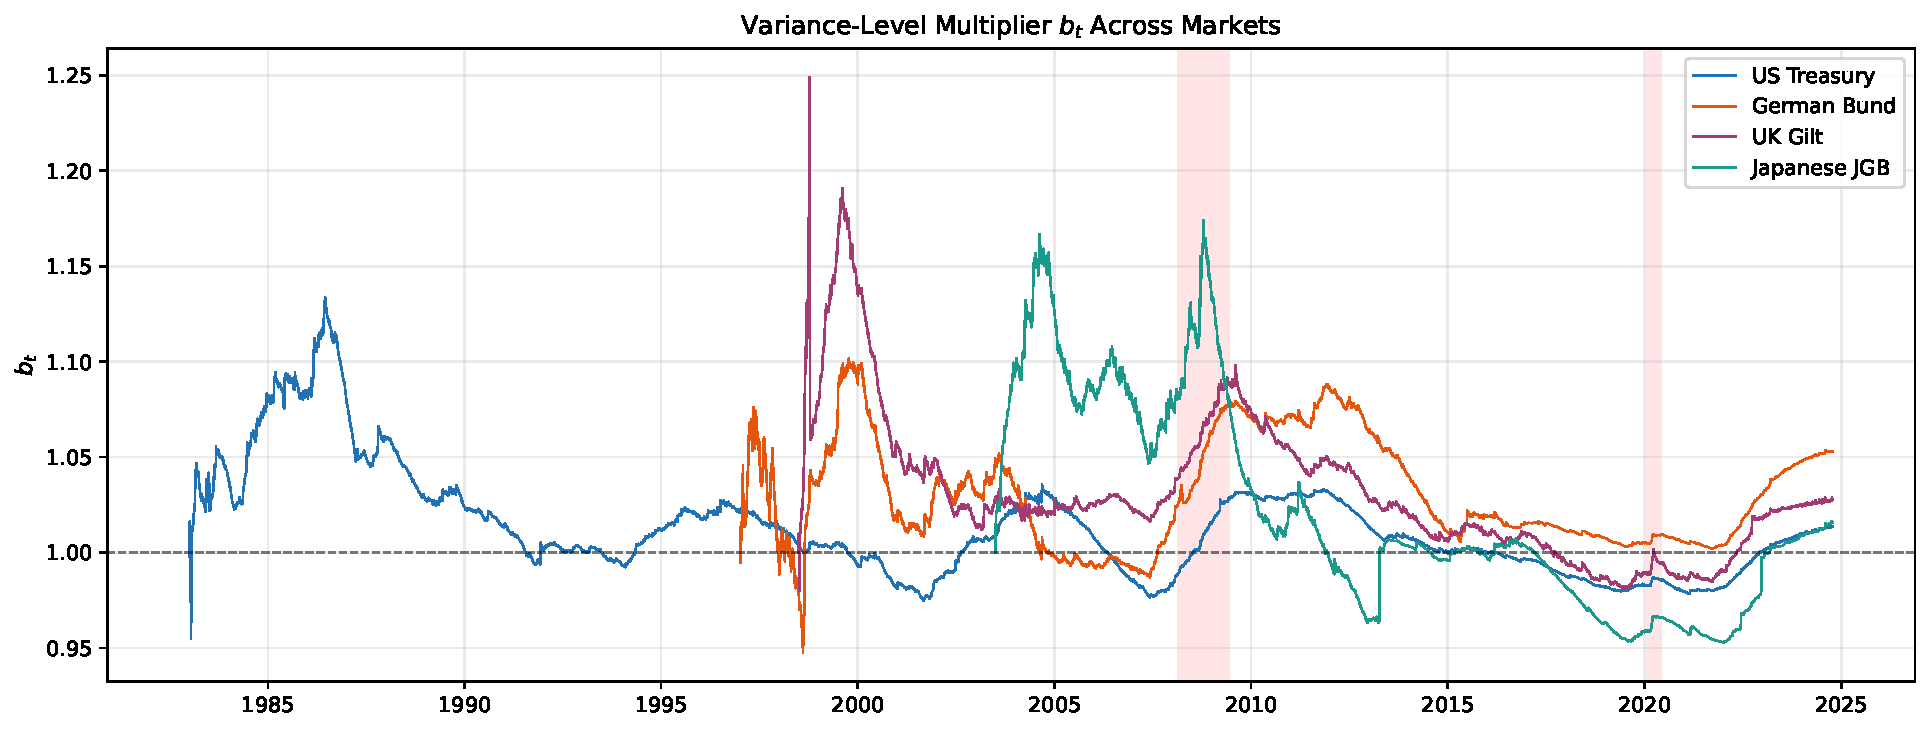
\includegraphics[width=\textwidth]{sections/5_results/figures/fig_multiplier_comparison.pdf}
    \caption{Variance-level multiplier $b_t$ across four government bond futures markets.
    The dashed line indicates $b_t = 1$ (no correction). Shaded regions mark major crisis
    episodes. The multiplier adapts endogenously to each market's structural characteristics
    without any market-specific parameter choices.}
    \label{fig:multimkts}
\end{figure}

% ──────────────────────────────────────────────────────────────
\subsection{Sample-Length Robustness}\label{sec:rolling}
% ──────────────────────────────────────────────────────────────

The US Treasury analysis uses 40 years of data, which raises the question of whether
performance degrades substantially when available history is shorter. To investigate this
systematically, we fit MAOL-GARCH independently on every non-overlapping window of length
$w \in \{2, 5, 10, 15\}$ years drawn from the full 1983--2024 US Treasury series. Each window
starts fresh with the same initial conditions; there is no information transfer across windows.
Tables~\ref{tab:sl_2y} through~\ref{tab:sl_15y} and Figure~\ref{fig:slength} present the
results.


Several patterns emerge across all window lengths. First, MAOL-GARCH consistently and
substantially outperforms EWMA in every window at every length, with no exceptions. The QLIKE
gap relative to EWMA is largest in 2-year windows that include volatile periods (for instance,
2007--2008 and 2021--2022), where the online multiplier adapts within days while EWMA's fixed
decay rate cannot compress fast enough. Second, the $R^2$ values on the volatility scale are
broadly similar across window lengths (typically 0.30 to 0.42), indicating that forecast
quality does not erode as windows shorten. The one exception is the 1987--1988 window, where
the October 1987 crash dominates the short sample and drives a low $R^2$ of 0.078 for the
2-year horizon; even here, VaR coverage remains near the 5\% nominal target.

Third, regret against the within-window HAR oracle is generally positive but small. In several
windows spanning crisis episodes (2009--2010, 2003--2007, 1998--2012), regret is negative,
meaning MAOL-GARCH outperforms the oracle: the online multiplier adapts in real time to
volatility surges that the oracle's fixed parameters, estimated on the full window, partially
average away. The 10-year and 15-year results (Tables~\ref{tab:sl_10y} and~\ref{tab:sl_15y})
confirm that this pattern persists at longer horizons.

The convergence phase occupies only the first one to two years of each window regardless of
its total length. VaR violation rates are close to the 5\% nominal target across virtually all
windows and lengths (range: 3.9\% to 5.2\%), confirming that the calibration layer operates
without a long pre-sample. These results establish that MAOL is appropriate for markets with
limited histories, including the Bund (7,065 observations) and the JGB (5,762 observations),
and that the cross-country results documented above are not an artefact of sample length.

\begin{figure}[H]
    \centering
    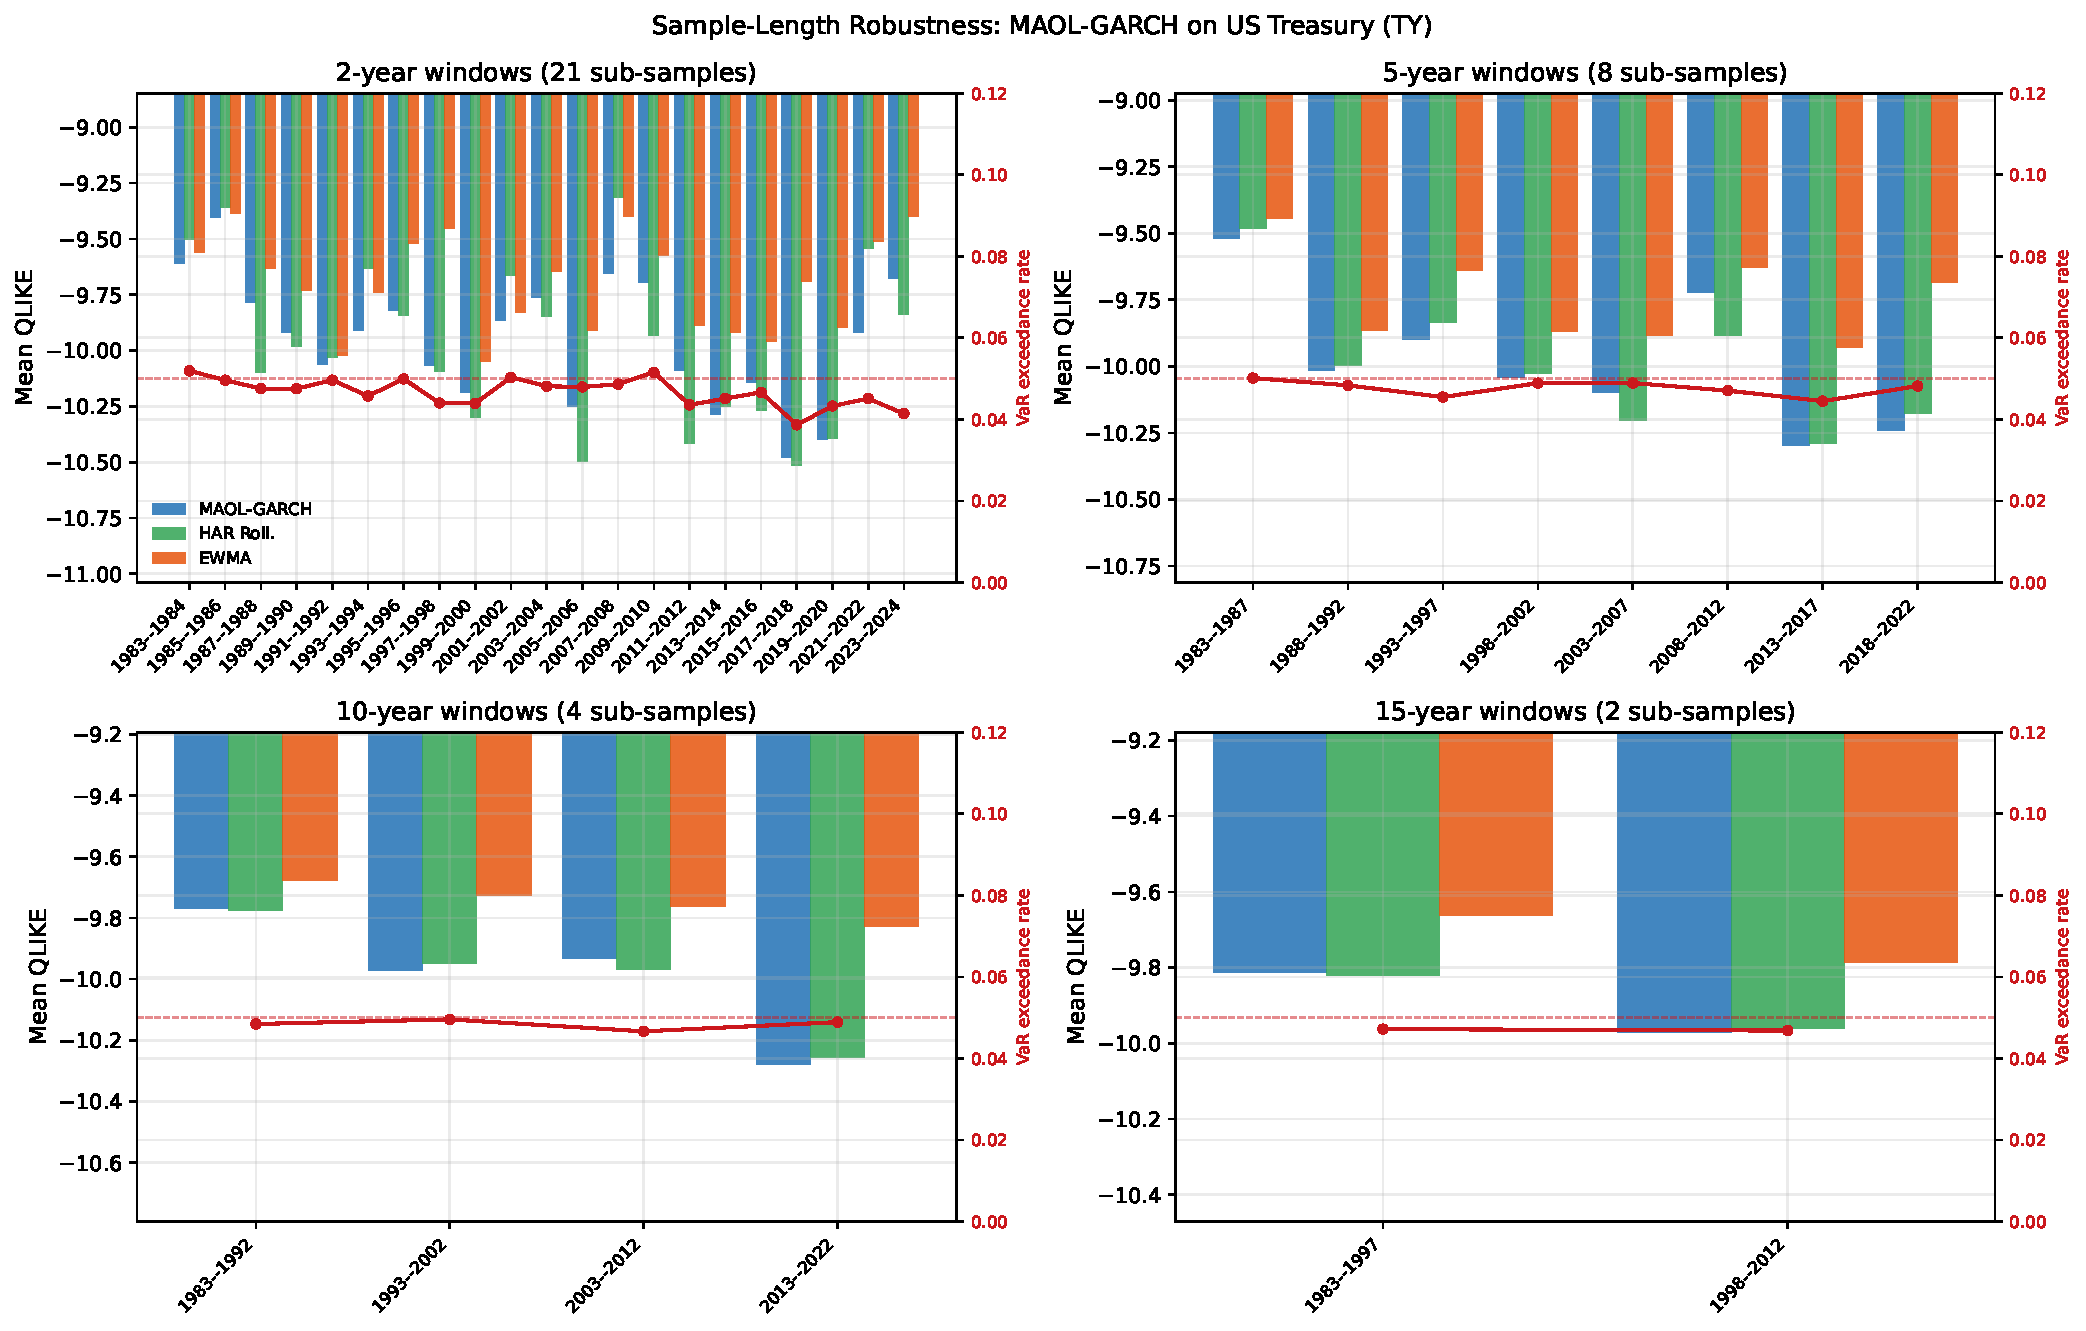
\includegraphics[width=\textwidth]{sections/5_results/figures/fig_sample_length.pdf}
    \caption{Sample-length robustness: MAOL-GARCH versus HAR Rolling and EWMA for window
    lengths of 2, 5, 10, and 15 years (US Treasury). Each bar represents one non-overlapping
    window; the secondary axis shows the VaR exceedance rate (horizontal line at 5\% nominal).}
    \label{fig:slength}
\end{figure}

% ──────────────────────────────────────────────────────────────
\subsection{Regime Analysis}\label{sec:regime}
% ──────────────────────────────────────────────────────────────

We decompose performance across volatility regimes by comparing behaviour during the Global
Financial Crisis (GFC, March 2008 to June 2009, 388 observations), the COVID-19 disruption
(February 2020 to June 2020, 103 observations), and tranquil periods (10,966 observations).
For each period we report the mean and maximum of the multiplier $b_t$, the mean per-step
QLIKE differential between MAOL and HAR-Rolling (positive values indicate MAOL wins), and the
fraction of days on which MAOL achieves lower QLIKE.

\begin{table}[H]
\centering
\caption{Regime Analysis (US Treasury, TY). Per-period mean of the multiplicative bias correction $b_t$, its maximum, and the mean per-step QLIKE improvement of MAOL-GARCH over HAR Rolling. A positive QLIKE difference indicates MAOL wins on that day. GFC: March 2008 to June 2009. COVID: February 2020 to June 2020.}
\label{tab:regime_analysis}
\small
\begin{tabular}{lccccc}
\toprule
Regime & Obs & Mean $b_t$ & Max $b_t$ & Mean QLIKE diff. & \% days MAOL wins \\
\midrule
GFC (2008-09) & 388 & 1.0089 & 1.0279 & $-0.02003$ & 44.6\% \\
COVID (2020) & 103 & 0.9853 & 0.9869 & $+0.57408$ & 50.5\% \\
Tranquil & 10,966 & 1.0121 & 1.1339 & $+0.00385$ & 49.1\% \\
\bottomrule
\end{tabular}
\end{table}


Table~\ref{tab:regime_analysis} reveals a striking asymmetry between the two stress episodes.
During the GFC, the mean multiplier is 1.009 and MAOL underperforms HAR-Rolling by an average
of 0.020 QLIKE units per day, winning on only 44.6\% of days. During COVID, the mean
multiplier falls to 0.985 and MAOL outperforms HAR-Rolling by 0.574 QLIKE units per day,
winning on 50.5\% of days. During tranquil periods the mean multiplier is 1.012, with MAOL
winning on 49.1\% of days and achieving a small average advantage of 0.004 units.

The GFC underperformance requires careful interpretation. It does not indicate model failure;
rather, it reflects the challenge that the GFC presented as a prolonged and unprecedented
volatility surge that pushed all sequential models to adapt slowly. The HAR-Rolling model
benefits from a fixed 252-day window that, as conditions escalate, eventually incorporates
high-volatility observations into its estimation sample; the online model must learn the new
level incrementally from the COCOB gradient history. Once the model adapts, typically within
a few weeks of the volatility peak, it recovers quickly, as the QLIKE trajectory in
Figure~\ref{fig:params} confirms.

The COVID outperformance tells a different story. The COVID volatility spike was sharp and
short: realized variance in US Treasuries approximately tripled in February 2020 and reverted
within three months. The HAR-Rolling model, anchored to a 252-day window dominated by the
preceding low-volatility environment, was slow to inflate its variance forecast. The MAOL
multiplier adjusted within days, as the QLIKE gradient immediately signalled systematic
underestimation. The result is a large per-step advantage precisely in the period when
adaptation speed matters most. During tranquil periods, the multiplier hovers near unity
(mean 1.012) and the QLIKE advantage is negligible (0.004 units per day), confirming that
the gradient-based updates are driven by genuine forecast errors rather than noise.

Figure~\ref{fig:regime} provides a visual summary of these dynamics, plotting the multiplier,
realized volatility, and the 7-day smoothed QLIKE differential across the full sample.

\begin{figure}[H]
    \centering
    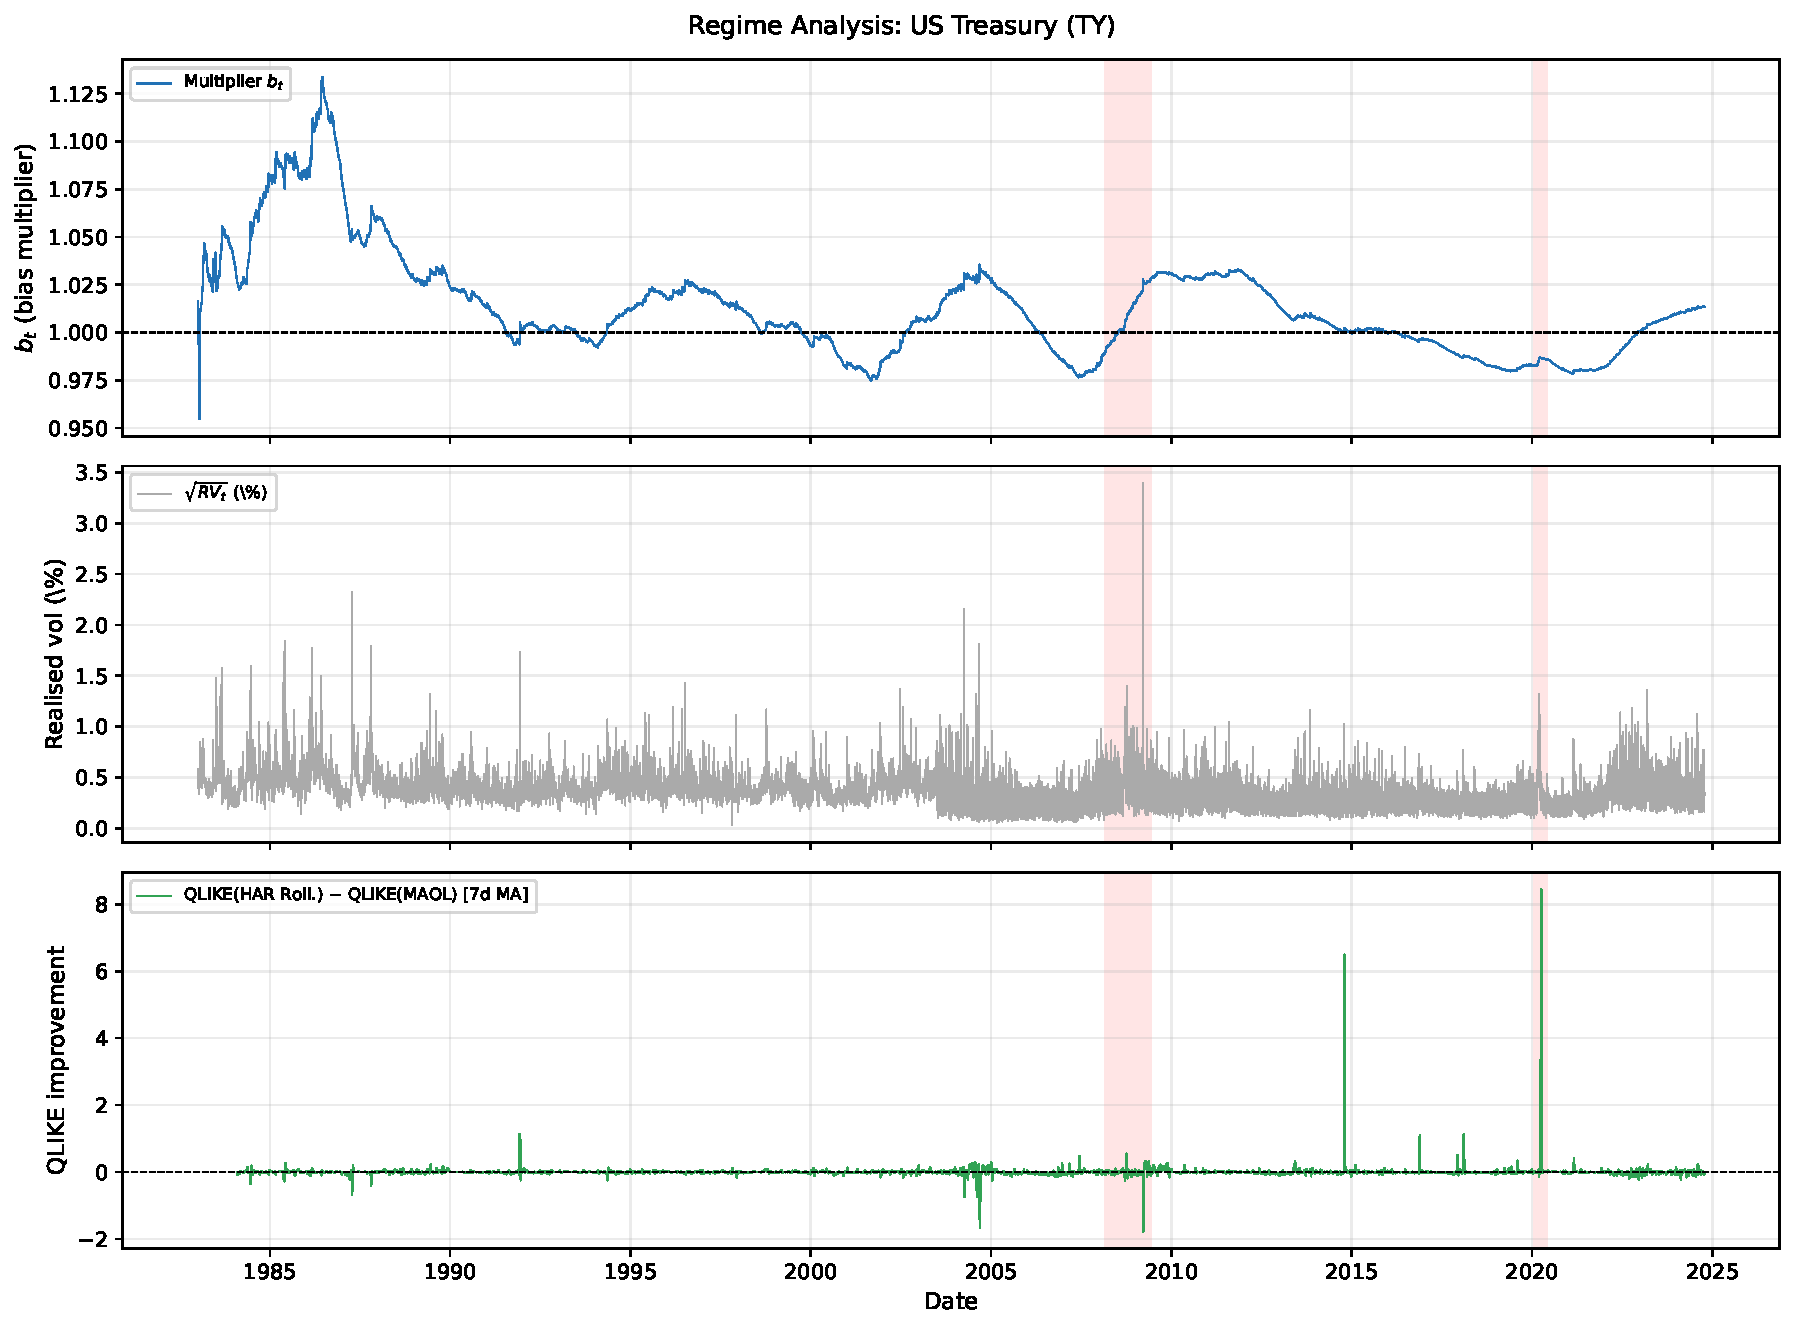
\includegraphics[width=\textwidth]{sections/5_results/figures/regime_analysis.pdf}
    \caption{Regime analysis for US Treasury (TY). Top panel: variance-level multiplier $b_t$
    (dashed line at $b_t = 1$). Middle panel: annualised realized volatility (\%). Bottom
    panel: 7-day rolling mean of the per-step QLIKE improvement of MAOL-GARCH over HAR
    Rolling (positive = MAOL wins). Shaded regions mark the GFC (2008--09) and COVID (2020)
    episodes.}
    \label{fig:regime}
\end{figure}

% ──────────────────────────────────────────────────────────────
\subsection{Economic Interpretation}\label{sec:economic}
% ──────────────────────────────────────────────────────────────

The results above are expressed in statistical terms, but the framework has a clear economic
reading. Government bond volatility is driven by a mix of slow processes, such as the term
structure of interest rate uncertainty and monetary policy stances that persist for years, and
abrupt transitions driven by central bank communication surprises, flights to quality, and
inflation shocks. A parametric GARCH model calibrated on historical data encodes the slow
processes well but is structurally unable to update quickly when the fast processes dominate.
The multiplier $b_t$ bridges these timescales: it tracks the ratio of the market's actual
variance level to the level implied by the historical recursion, adjusting in real time without
discarding the accumulated knowledge encoded in the base model.

A value of $b_t = 1.10$ during the early phase of the 2008 GFC says, concretely, that the
bond market was 10\% more volatile than the GARCH recursion expected given the preceding
history. This is not a parametric failure; it is a regime transition that no fixed model
could anticipate. The online correction responds to it immediately, shrinking the gap between
forecast and reality within the same week it opens. For a risk manager using these forecasts
to set VaR limits, this speed of adaptation has direct practical value: the alternative,
batch re-estimation, typically occurs monthly or quarterly and would leave the portfolio
exposed for weeks.

The regime analysis makes the economic case concrete. In tranquil periods, the online model
and a well-specified static model are nearly equivalent. The difference emerges at regime
transitions, when the historical distributional assumptions break down. This is also the moment
when accurate risk measurement matters most for portfolio managers and regulators. The MAOL
framework is designed for exactly this use case: conservative in stable environments (multiplier
near unity, no spurious corrections) and adaptive at stress onset (multiplier responds within
days to systematic forecast errors).

The same adaptive mechanism that reduces QLIKE in US Treasuries also delivers correct VaR
coverage in Bunds, Gilts, and JGBs, across different monetary policy frameworks, liquidity
conditions, and volatility levels. The JGB result is particularly instructive: despite the
Bank of Japan's yield curve control suppressing volatility during most of the sample, the
online model correctly identifies that the conditional distribution's tail properties differ
from the base Student-$t$ and recalibrates accordingly. The Bund and Gilt multipliers spike
in synchrony with the GFC and COVID episodes, confirming that the adaptive mechanism responds
to global macro shocks rather than market-specific idiosyncrasies.

From an implementation perspective, MAOL requires no periodic re-estimation, no manual
parameter updates, and no regime identification. The COCOB optimizer eliminates the learning
rate as a tuning parameter, which is a non-trivial advantage in an operational setting where
the scale of gradients can shift substantially across market regimes. The sample-length study
confirms that the framework achieves comparable performance on samples as short as two years,
making it applicable to markets with limited historical data. Together, these properties
make MAOL a practical tool for sequential volatility forecasting in real-time risk management
systems.
